\chapter{Implementation of a Prototype for Distributed-UI Scenarios}\label{chapter:impl}
In chapter \ref{chapter:design}, a conceptual design for a single-user video recommendation application in a distributed UI environment was introduced. The goal of this design is to improve the recommendation process by leveraging the capabilities of the different platforms along which the UI is distributed. To put the design to test, a high-fidelity prototype was developed to mimic the functionalities of the complete system, hence, making it possible for evaluation through real user experience. A subset of the suggested distribution aspects with respect to the different distribution dimensions (user, task, time, space..etc) which was presented in the design chapter is selected for implementation. The selection criteria of the scenarios to be implemented was to select the ones that would be verifiable using the setup we had in mind for the user study. Since our user study involves only single user, scenarios that need more than  one user at a time to verify (such as distributing a favourites list between users) where left out from the implementation. Moreover, our focus is the distribution of the post-recommendation phase. Therefore, tasks and activities involved in the pre-recommendation are not implemented. A recommendation engine is also not included since the focus of the study is not with recommendation generation. Instead, we provide the user with a set of pre-selected video items. This section provides the set of functionalities included in the prototype, as well as an explanation of implementation details of the prototype, together with explanations for the rationale behind using the frameworks, programming languages, platforms and tools used in the course of implementing this prototype. 
 
\section{Prototype Versions and Functionalities}
The prototype of a video recommendation application was implemented as a mobile application. The implementation of the prototype was done with the user study in mind. Since the planned study is designed to test our hypothesis of whether the UI distribution of such a system is of added value, the study is based on comparing user feedback on using two different versions of the prototype: a distributed version and non-distributed one. This section explains the difference between each version through describing the different use cases of each version.
\subsection{Non-Distributed Vs. Distributed Prototype Versions}
The first steps of designing the prototype was to think of the different versions in terms of user and system functionalities that would be available through each version.
The non-distributed version of the application is deployed as an iOS mobile application only. The distributed version is distributed along 2 different platforms: the iOS mobile phone and a LD screen attached to a PC. The iOS application in both versions are fundamentally similar except for the use cases that were selected for distribution. Figure shows the different use cases in the distributed and non distributed versions.
\begin{figure}[h]
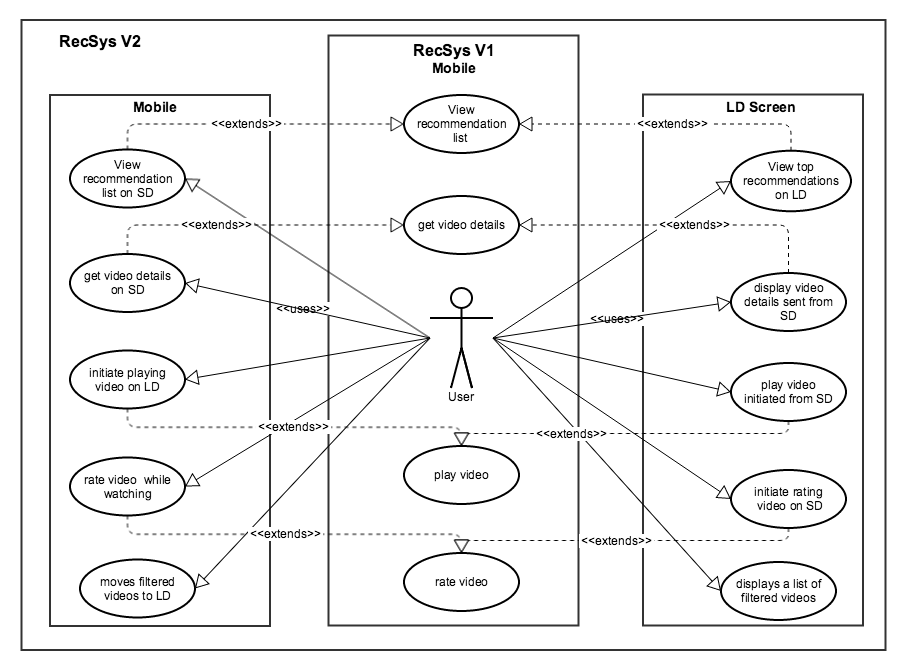
\includegraphics[width=0.8\textwidth, center, center]{figures/usecase}
\caption{Use Case Diagram of MiRec(RecSys V1) and DiRec(RecSys V2).}
\label{fig:figure42}
\end{figure}
\subsection{Use Cases and Functionalities}
As shown in figure \ref{fig:figure42}, the main use cases for the first non-distributed versions of the prototype are depicted by the inner rectangle. They are described as follows:
\begin{itemize}
  \item The user should be able to view a list of all recommended videos. The list should be categorized with respect to the video topic or related topics.
  \item The user should be able to select a video and get more detailed information on the selected video.
  \item The user should be able to play the selected video on his/her mobile phone.
  \item The user should be able to rate the played video after watching.
\end{itemize}
The use cases of the distributed version of the prototype are given in figure \ref{fig:figure42} by the outer rectangle and grouped by the mobile and the LD components of the systems. The functionalities are thought of as special cases, or extensions, of the first version:
\begin{itemize}
	\item As opposed to getting a list of recommended videos on the mobile, the user should be able to get both a list recommend videos on the mobile phone (SD) as well as an overview of the top recommended video items on the LD. Both views should be presented in parallel on triggered by the other. 
	\item Getting the video details should be available on the SD. Additionally, the user should be able to transfer the details of the video to be displayed on the LD using a simple gesture. 
	\item The video consumption/playing is distributed between the two displays. The user should be able to select the video on the mobile phone and with a simple gesture, should be able to trigger playing the video on the LD.
 \item Once the video starts playing on the LD, the user should be prompted with the rating view on the SD. Both functionaries (playing and rating) could be done in parallel.
 \item The user should also be able to filter his/her choices of videos. This use case is also distributed along both devices. The user should be able to apply a gesture on the selected video on the SD and get this video to be transferred to the LD. By the end of this process, the user should be able to be presented of all filtered videos on the LD. 
\end{itemize} 
     
\section{Overview System Architecture}
The user is presented with a mobile device and an LD screen through which the interaction with the system is possible. Figure \ref{fig:figure41} shows a deployment diagram of the different system components. The system is composed of two separate applications running on two different platforms with a communication layer between them: an iOS application running on an iPhone mobile device, and a python application running on PC connected to an LD screen.  A number of artifacts are needed to run both applications, as depicted by figure \ref{fig:figure41}: An iPhone mobile device with the .ipa of the mobile app installed on it, and on the LD side, a desktop application, with the Python runtime environment installed, should have the .py UI application installed on it. The PC is connected through an HDMI cable to an LD screen. Both the mobile device and the PC should be connected to the same network for communication.
    
This section provides implementation details of each application as well as the layer that channels communication between them.    
\begin{figure}[h]
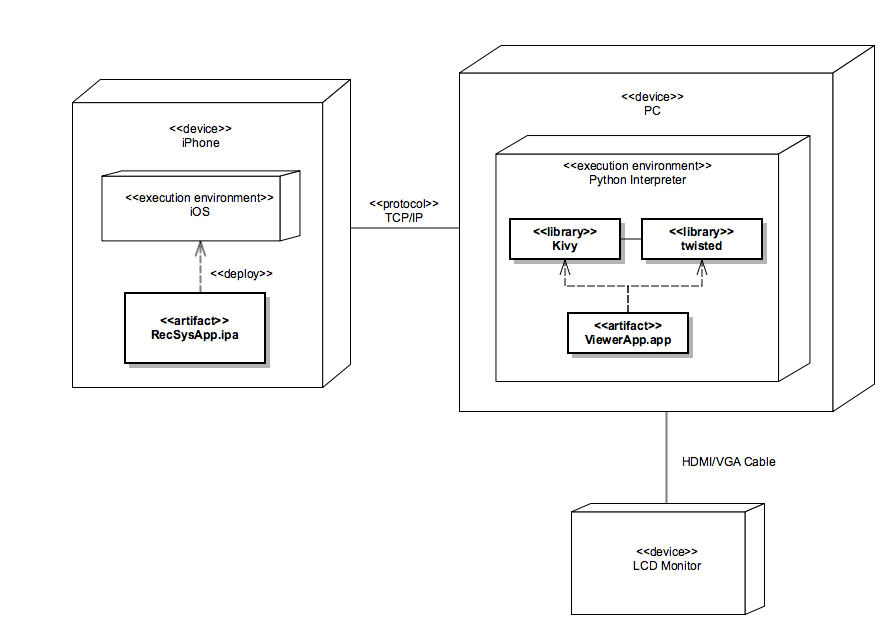
\includegraphics[width=0.8\textwidth, center, center]{figures/deployment}
\caption{Overview Architecture of The System's Components.}
\label{fig:figure41}
\end{figure}

\subsection{Mobile Application}
The first step of implementation, after deciding on the set of functionalities that should be present in each version as described in the previous section, was to start with creating a storyboard for the first non-distributed version of the application. As mentioned, the mobile application is implemented as a native iOS application running on iPhone mobile device. The app was written in Objective C, and uses Apple's iOS SDK 8.4 and basic frameworks for the implementation of most of the functionalities, except for some third party APIs that will be mentioned later. Xcode version 6.4 was used in implementing and preparing the distribution version of the app.\\
The second distributed version of the app did not include much variation when it comes to most of the views and navigation available in version one. Therefore, the storyboard was not changed to a great extend in the second version. The main variation in the distributed version was included on the functionalities implementation which will be discussed in later sections.
  
\subsection{LD Screen Application}
The design of the LD application started by investigating the different technologies available that support the functionalities we needed to implement as a desktop application with a graphical UI. What needed to be supported was means to build a graphical UI that enables user interaction, as well as the capability of playing and controlling video files. Axiomatically, easy means for communicating with the iPhone app that would allow for implementing the UI distribution is a key feature. At first, implementing a Mac OS X desktop application seemed as the best option. However, as we aimed for a more potable option that also support rapid prototype development. Hence, Python based application was rather thought of for being highly portable and light weight for development for this special purpose prototype. Hence, for the implementation of the desktop application, we use the Kivy; an open-source Python based library that was developed with the creation of innovative user interfaces and rapid development as its primary edge. Kivy provides the tools needed to build graphical UI within its basic library, as well as libraries needed for video playback. The graphics engine is built over OpenGL ES 2, using a fast graphics pipeline. It also supports third party libraries that would be easily integrated for network communication with the iOS application as described in the following section. Kivy's portability makes it possible to run the developed application on any platform: Windows, Linux, OS X, iOS Android, which provides a length of variety on the selected platform for deployment.   
 
\subsection{Communication Layer}
The development of applications that use distributed UI components along different platforms is not made possible through special frameworks or tools. Therefore, it is up to every application developer to build a solution that makes the distribution requirements achievable. In our model, we rely on a message passing protocol between the iOS mobile application and the desktop application. This message passing  work as commands between the two applications to execute certain tasks (e.g. play video, show details, etc ...). This communication needs to be light-weight and quick to prevent any latency. One of the design goals is to provide seamless distribution of the UI between the two displays, such that the user would be able to carry out the tasks as efficiently as if the task was not distributed in the first place. Hence, the network communication between the iOS application and the Kivy desktop application is chosen to done through socket communication over TCP/IP. The desktop application, besides running its main functionalities, also runs as a custom TCP server that listens to connections on a given TCP socket. The client in this scenario is the iOS application which initiates connection once the app is running on a specific port and IP address. Using TCP sockets for communication makes the implementation of the communication layer independent on a web server, which also means a freedom to choose the implementation language for the server. Moreover, using TCP sockets provides light-weight means for building a lean and efficient protocol for communication through which we could send exact messages that needs to be sent between the applications.\\
To build the network protocol and the custom server on the desktop side Twisted is used. Twisted is a Python networking framework that makes network communication easier than using Python's basic networking library. Kivy also comes with support for Twisted.\\
On the iOS side, the CFStream API is used to establish a socket connection and, with the stream object created as a result, send data to and receive data from the custom python server on the desktop side.

\section{Implementation of Distributed Scenarios}

This section provides details of the implementation of the high-level functionalities of the distributed version of the prototype through the explanation of how the different described scenarios were implemented. It is worth noting that the implementation of such scenarios were taking place iteratively; some the mobile application functionalities were implemented and then modified when new requirements were added as more scenarios were added or changed. Also, the implementation of the server desktop side was done in parallel to the implementation of the iOS side in a continuous integration manner in order to ensure both sides integrate correctly. It is also worth mentioning that the data gathered for this prototype was done using a python script that scrapped TED.com for video cast files' urls and information including detailed description, speakers, dates, images and duration. A total of 73 video casts information was gathered from different topics. Data was not saved in a database, however, was duplicated as XML-based property list files on both the iOS and desktop sides. For the sake of the prototype, fast access of data was needed, and since the data fits more a dictionary representation and has no relational aspect, creating a separate database was thought of as redundant. Also duplication of property list resource on both sides is through to be more efficient than having to access a shared resource despite of the update overhead that would be necessary if any of the copies were to be edited.\\
Appendix \ref{chapter:appendA} provide a high-level class diagram for both iOS and desktop applications for details.

\subsection{Establishing Connection}
Initialising TCP sockets communication between the iOS app and desktop app is the first step. Since the desktop app works also as the server, this step has to start by calling Twisted reactor on the server side to start its main loop and wait for connections from the iOS client. The specific IP address and port for communication are hardcoded in the application for simplicity, so that no pairing mechanism would need to be implemented. Once Twisted is started and added successfully to the main loop of the Kivy application, the desktop app enters the Waiting for Connection state. Figure shows the welcome screen that indicates that the server is running and waiting for connection.\\

On the iOS app side, a Communication Manager singleton class is initialised in the App Delegate once the application finishes launching. In the Communication Manager init method, NSStreams (input and output) are created after a connection with the server is requested at the given IP address and port which are also hardcoded with the same values as the desktop application. Once a connection is made successfully (given that the server is already running), Communication Manager initialises the messaging protocol with the following messages:
\begin{itemize}
	\item \textbf{\textit{open:home}} for opening home view on LD. 
	\item \textbf{\textit{play:<videoID>}} for playing a video with id \textit{videoID} on LD.
	\item \textbf{\textit{detail:<videoID>}} for redirecting details of video with id \textit{videoID} to LD.
	\item \textbf{\textit{filter:<videoID>}} for redirecting video with id \textit{videoID} for filtering on LD.
	\item \textbf{\textit{rate:<videoID>}} for rating video with id \textit{videoID} on SD.
\end{itemize}
As shown, the message payload consists of a command part and a value part separated with a colon. In case video information is needed to be redirected, only the video id is sent and not the actual content of the video. This way, we minimise the overhead of communication by passing light-weight messages that are sufficient for performing the tasks.\\
At this point, the desktop server enters the Ready State and awaits for receiving messages from iOS client.

\subsection{Loading Video Data}
After the connection is established successfully and the protocol is initialised, loading of video data is done on both sides. On the iOS side, a data model class \textit{Video} is created to hold video details. For each video object, the following attributes are loaded: id, title, description, speaker, duration, year, and topic.
Data is loaded in memory once from the property list by a Data Manager as Video objects. On the desktop side, the property list is also loaded in a read-only structure.       
\subsection{Presentation of Recommended Videos}
The first distributed scenario that user is presented with is the presentation of a Home view which holds the recommended video items. On the iOS side, the videos are presented as a TableView list, which also acts as a master view to a details view  which is loaded on clicking one of the items. Fine granularity of detail is presented to the user on the iOS side. The list is divided into sections showing different categorisation of the recommended content titled with explanations as such: \textit{Top Picks for <User>}, \textit{Because You Liked <Category>}, \textit{Top Rated in <Category>}, \textit{You Might Also Like}, etc... This type of explanation is hardcode and not based on actual recommendation logic but was added to mimic real recommendations. Beside the Home view, a side menu enables the user to get a list of all available categories for further details. Selecting one of the categories would also open list view similar to that of Home however specific to that category.\\
Simultaneously, on loading the home view on iOS, \textbf{\textit{open:home}} is sent to the sever to load the home view on the desktop side. On receiving this message, the server loads a Grid layout with an overview presentation of recommended videos in different sizes which indicate the recommendation score. Figure \ref{fig:figure43} shows the different screens shown on each side.
\begin{figure}
    \centering
    \begin{subfigure}[b]{0.6\textwidth}
        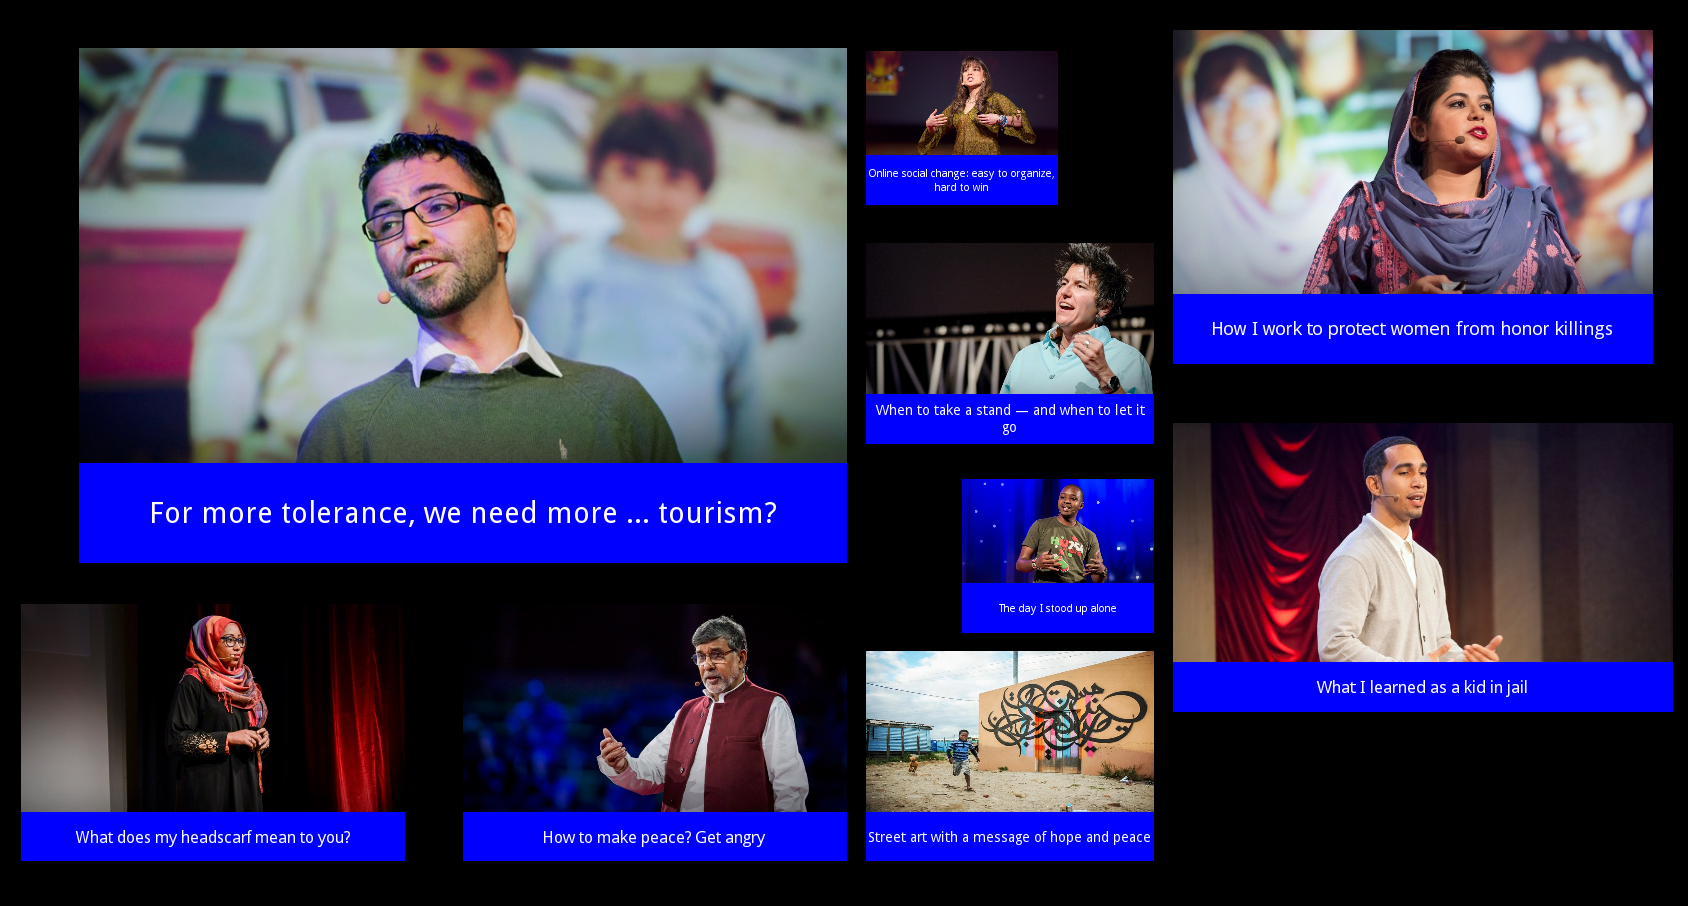
\includegraphics[width=\textwidth]{figures/homeLD}
        \caption{Home view on LD display.}
        \label{fig:figure43a}
    \end{subfigure}
    ~ %add desired spacing between images, e. g. ~, \quad, \qquad, \hfill etc. 
      %(or a blank line to force the subfigure onto a new line)
    \begin{subfigure}[b]{0.3\textwidth}
        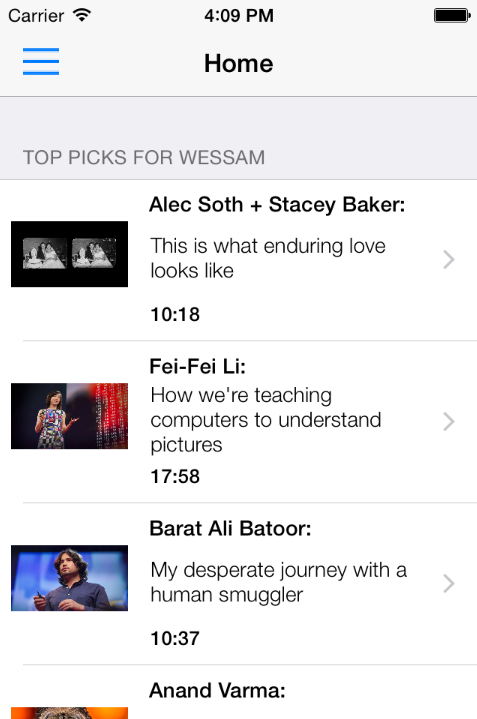
\includegraphics[width=\textwidth]{figures/homeSD}
        \caption{Home view on SD/mobile display.}
        \label{fig:figure43b}
    \end{subfigure}
   \caption{Presentation of Recommended Videos on SD and LD displays}\label{fig:figure43}
\end{figure}
\begin{figure}
    \centering
    \begin{subfigure}[b]{0.6\textwidth}
        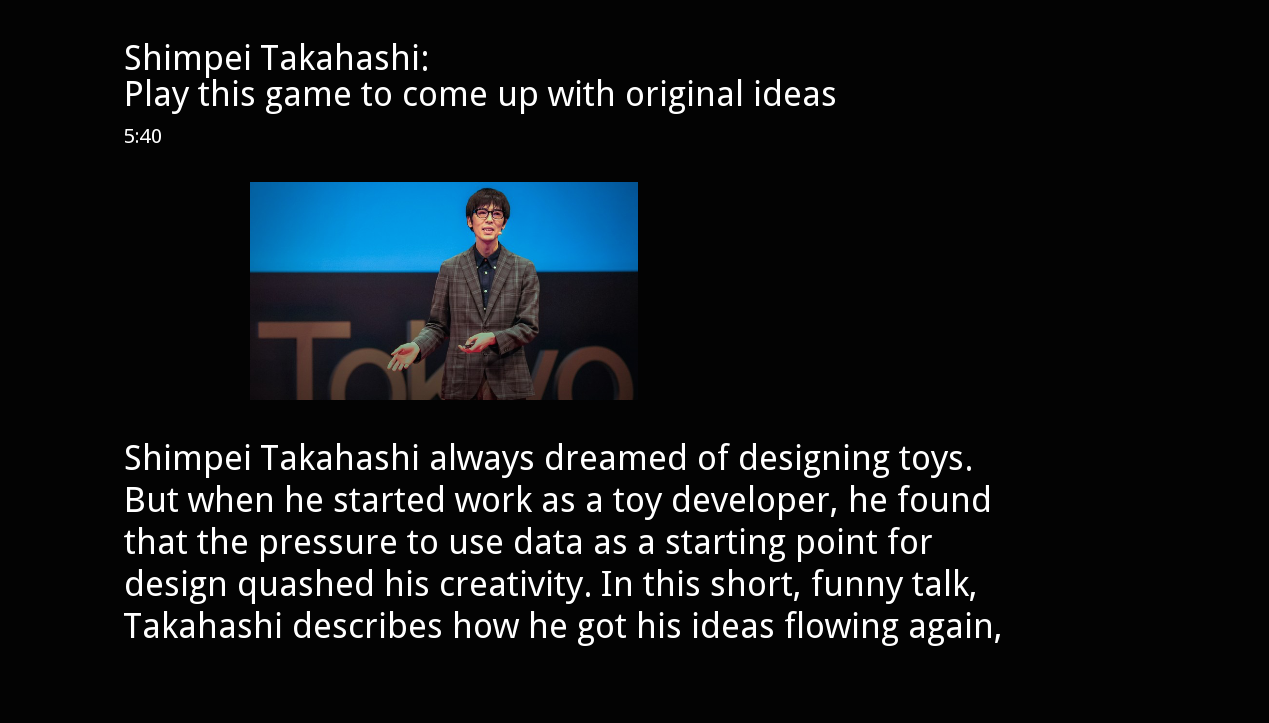
\includegraphics[width=\textwidth]{figures/detailsLD}
        \caption{Showing video details on LD}
        \label{fig:figure44a}
    \end{subfigure}
    ~ %add desired spacing between images, e. g. ~, \quad, \qquad, \hfill etc. 
      %(or a blank line to force the subfigure onto a new line)
    \begin{subfigure}[b]{0.3\textwidth}
        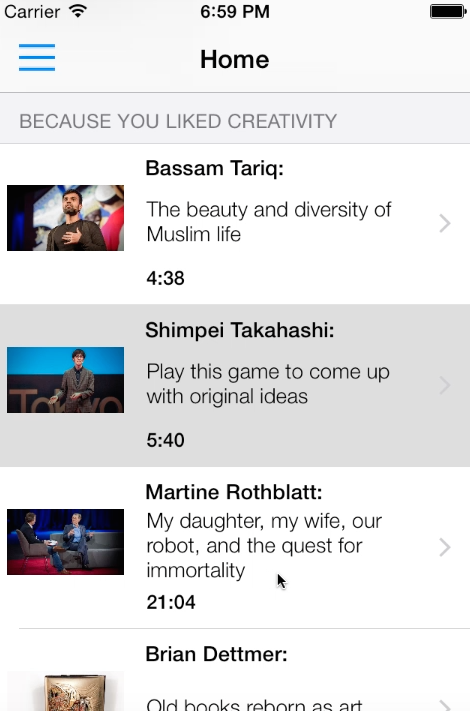
\includegraphics[width=\textwidth]{figures/swipeleftSD}
        \caption{Swipe right gesture on table view cell.}
        \label{fig:figure44b}
    \end{subfigure}
   \caption{Presentation of Video Details}\label{fig:figure44}
\end{figure}

\subsection{Presentation of Video Details}
Getting details of a video is started on the iOS side by clicking on a given video in the Home list which presents a details view. The details viewew is similar in both the distributed and undistributed versions of the prototype. Moreover, viewing the details of the video on the LD is possible by performing a left swap gesture on the tableview cell of the video item on the iOS side. After performing the gesture, Communication Manager sends \textbf{\textit{detail:<videoID>}} with the specific video id. The desktop server receives and parses the sent message. For the command \textbf{\textit{detail}}, a layout is created, loaded, and filled with the content of the video details whole id was sent as the value part of the parsed message. After this operation is complete, the user is able to view details of the videos on both the SD and LD. Figure \ref{fig:figure44} depicts this scenario.
\begin{figure}
    \centering
    \begin{subfigure}[b]{0.3\textwidth}
        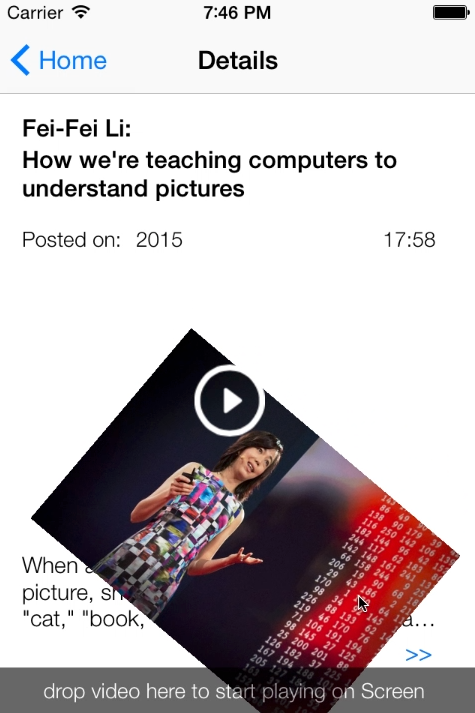
\includegraphics[width=\textwidth]{figures/playSDb}
        \caption{Pan gesture on video image}
        \label{fig:figure45a}
    \end{subfigure}
    ~ %add desired spacing between images, e. g. ~, \quad, \qquad, \hfill etc. 
    %(or a blank line to force the subfigure onto a new line)
    \begin{subfigure}[b]{0.3\textwidth}
        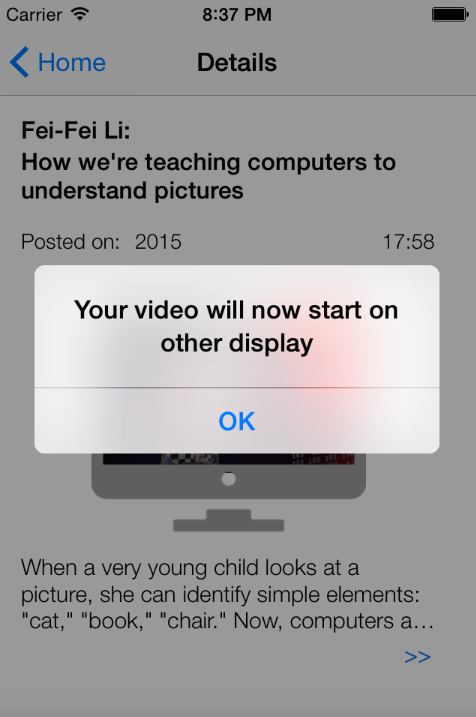
\includegraphics[width=\textwidth]{figures/playSDd}
        \caption{Notification alert to play transfer video to LD.}
        \label{fig:figure45b}
    \end{subfigure}
    \begin{subfigure}[b]{0.3\textwidth}
        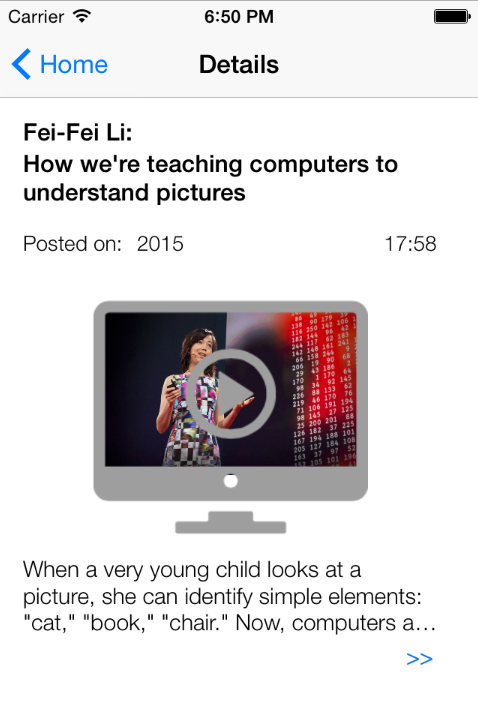
\includegraphics[width=\textwidth]{figures/playSDc}
        \caption{Indication that the video has started on LD}
        \label{fig:figure45c}
    \end{subfigure}
    \caption{Initiating video playing on LD}\label{fig:figure45}
\end{figure}
\subsection{Playing a Video}
The distributed scenario of playing a video (figure \ref{fig:figure45}, \ref{fig:figure46a}) is one that also starts at the iOS side. The user select a video from the list and then is directed to a details page. Inside the details page, besides view the video details, to play a video on the LD, the user simply taps and drags (panning) the image of the video presented in the centre of the screen towards the bottom of the screen. Figure shows a sample of this action. The panning gesture triggers sending a message to the desktop server \textbf{\textit{play:<videoID>}}, which send the play command and the selected video id to the server. The server receives and parses the message and loads an instance of a video player initialized with the video url. The video player starts streaming the content and displaying it on the attached LD screen. For playing and controlling the video kivy.uix.videoplayer package is used which is built-in in the Kivy library.\\ 
The non-distributed version of the prototype presents the user with a play button on top of the video image in the details page. On clicking the button, the video player is loaded as a modal view on top of the details view, where control and playing of the video is made possible on the mobile device. 
 
\subsection{Rating a Video}
In the distributed version of playing a video, starting the rating scenario is done once the player is started on the LD. The desktop sever sends a message \textbf{\textit{rate:<videoID>}} to the iOS app to display the rating view. Hence, the user could perform both tasks (rating and playing) in parallel. Figure \ref{fig:figure46b} shows the rating screen on the iOS side.\\
The same screen is shown in the non-distributed version however it is prompted after video playing on the SD ends or is stopped by the user.
\begin{figure}
    \centering
    \begin{subfigure}[b]{0.6\textwidth}
        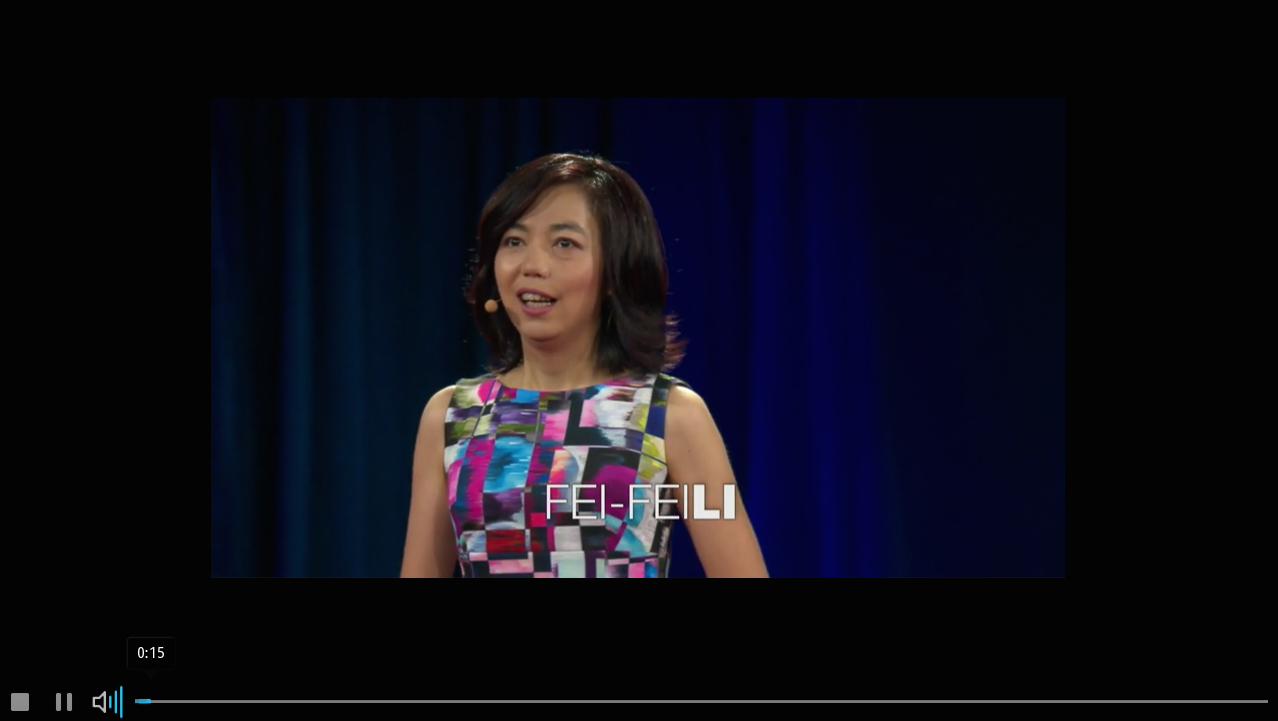
\includegraphics[width=\textwidth]{figures/playerLD}
        \caption{Video player started on LD}
        \label{fig:figure46a}
    \end{subfigure}
    ~ %add desired spacing between images, e. g. ~, \quad, \qquad, \hfill etc. 
      %(or a blank line to force the subfigure onto a new line)
    \begin{subfigure}[b]{0.3\textwidth}
        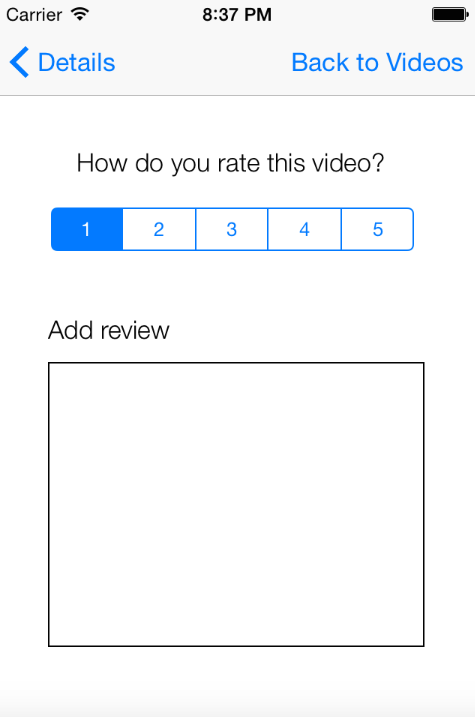
\includegraphics[width=\textwidth]{figures/ratingSD}
        \caption{Rating view started on SD on starting video player on LD}
        \label{fig:figure46b}
    \end{subfigure}
   \caption{Rating recommended videos on SD while playing a video on LD}\label{fig:figure46}
\end{figure}       
\subsection{Filtering Recommendations}
Optionally, the user is able to filter his/her choice of videos before deciding on which videos to play. Filtering is done by transferring the selected video from the recommendation list on iOS side to the LD application by performing a right swipe gesture on the video item table view cell. The swipe gesture triggers sending a message \textbf{\textit{filter:<videoID>}} from the iOS side to the desktop server side. When the message is received on the server side, the filter page is created as a grid layout and each transferred video is added as a new widget to the layout. Only the video image and title are shown on the LD. The user is also able to display more information for the page by clicking on the video image on the LD side. Figure \ref{fig:figure47} shows the filtering scenario as presented on the LD and SD.    
\begin{figure}
    \centering
    \begin{subfigure}[b]{0.6\textwidth}
        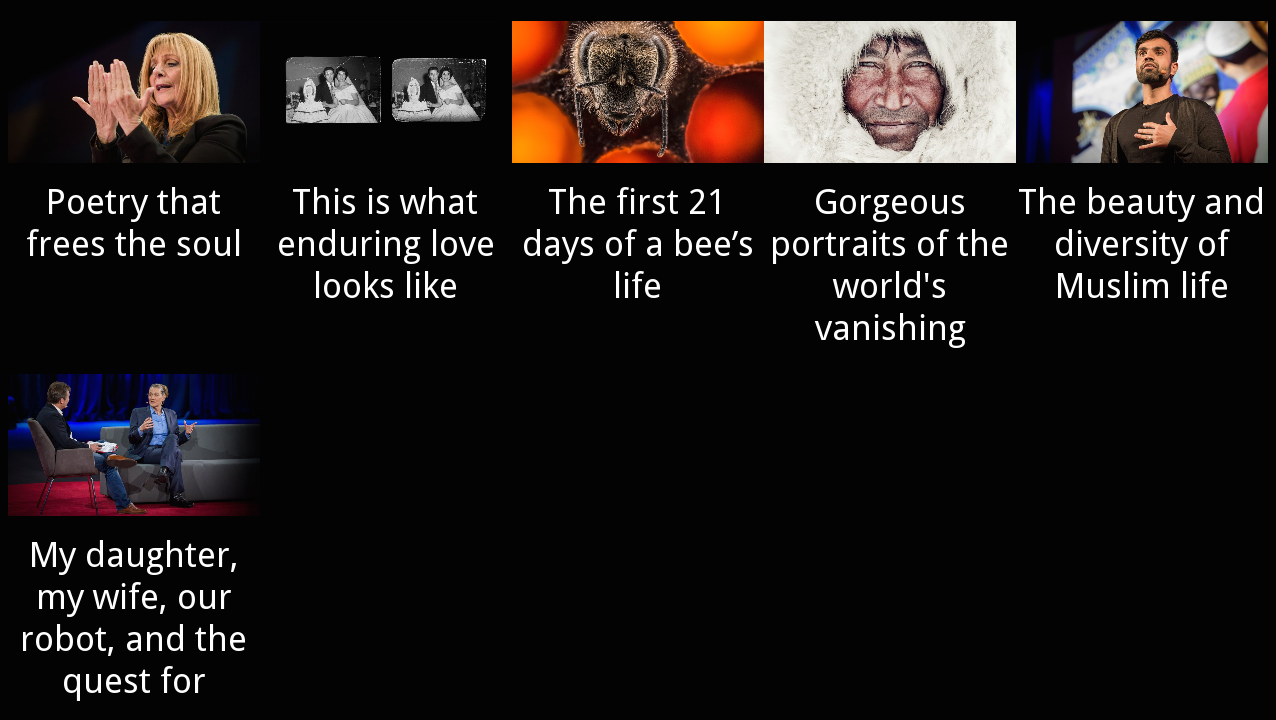
\includegraphics[width=\textwidth]{figures/filterLD}
        \caption{Filtering screen on LD}
        \label{fig:figure47a}
    \end{subfigure}
    ~ %add desired spacing between images, e. g. ~, \quad, \qquad, \hfill etc. 
      %(or a blank line to force the subfigure onto a new line)
    \begin{subfigure}[b]{0.3\textwidth}
        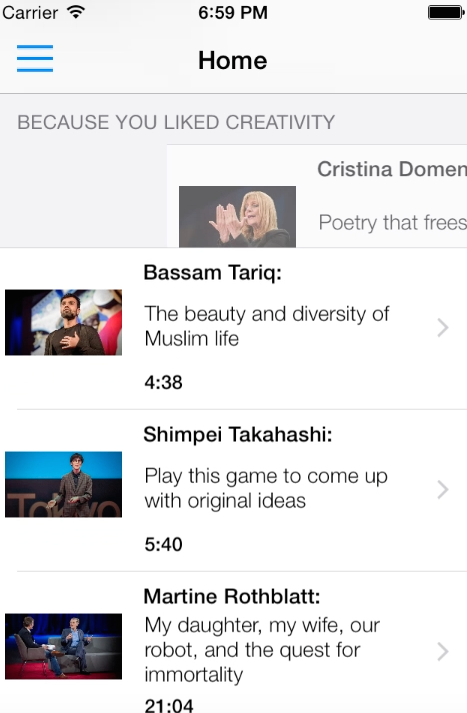
\includegraphics[width=\textwidth]{figures/swiperightSD}
        \caption{Right swipe gesture on table view cell on SD.}
        \label{fig:figure47b}
    \end{subfigure}
   \caption{Filtering Recommendations}\label{fig:figure47}
\end{figure}
  

 
         


